\documentclass[10pt,journal,twocolumn]{IEEEtran}
\usepackage[T1]{fontenc}
\usepackage{amsmath,amssymb,booktabs,graphicx,xcolor,siunitx,longtable}
\usepackage{tikz}\usetikzlibrary{shapes.geometric,arrows.meta,positioning,fit}
\usepackage{pgfplots}\pgfplotsset{compat=1.17}
\usepackage[numbers,sort&compress]{natbib}
\usepackage[hidelinks]{hyperref}
\renewcommand{\arraystretch}{1.18}
\title{\textbf{From Epoch-Level Illusion to Governed Deployment:\\ A Systematic Review of 50 Recent Works on EEG Epilepsy AI\\ and the Path to Governed, Agentic Deployment}}
\author{P.~Asthana,~\IEEEmembership{NeuroAI Research Group}}
\date{\today}
\begin{document}\maketitle

\begin{abstract}
\noindent Automated EEG seizure detection is reported above 95\% accuracy across hundreds of studies, yet deployment in patient-independent clinical settings remains rare. This systematic review of 50 works (2021--2026) argues that the discrepancy is rooted in an \emph{evaluation-honesty} gap: most reported accuracy is obtained under epoch-level cross-validation, which leaks subject-specific information. We synthesise the corpus along eight architecture families, five task formulations, six public datasets, and two evaluation regimes; quantify the epoch-vs-subject-wise gap (a companion empirical study finds a 53-point sensitivity collapse on an identical pipeline); and catalogue fifteen field-level gaps. We then propose a forward deployment architecture---multi-agent governance, retrieval-augmented explanation, Model Context Protocol tooling, and AIOps monitoring---that the surveyed literature omits. We position Responsible, Explainable, and Interpretable AI as first-class reporting metrics and release the curated corpus.
\end{abstract}

\noindent\textbf{Keywords:} EEG, epilepsy, seizure detection, systematic review, Leave-One-Subject-Out, data leakage, transformer, graph neural network, foundation model, responsible AI, retrieval-augmented generation, Model Context Protocol, AIOps.

\section{Introduction and Scope}
Epilepsy affects approximately 50 million people, and EEG remains the diagnostic gold standard \citep{ep241003385}. The last five years produced an explosion of deep-learning detectors \citep{ep250820535,ep251108861,ep260113234}, but two questions remain inadequately answered by the literature taken as a whole: (i) \emph{is the reported accuracy honest for unseen patients?} and (ii) \emph{what does a clinically deployable, governed system actually require beyond the model?} This review addresses both. Its scope is recent (2021--2026), peer-reviewed and pre-print EEG epilepsy AI, covering detection, prediction, onset localisation, type classification, and interictal-biomarker tasks across scalp, intracranial, and consumer-grade acquisition.

\textbf{Why another review.} Existing surveys catalogue architectures and datasets but rarely (a) frame evaluation honesty as the central validity threat, (b) treat Responsible/Explainable/Interpretable AI as measurable axes, or (c) specify the agentic, retrieval-grounded, governed deployment layer. This review does all three.

\section{Review Methodology}
We followed a PRISMA-style protocol. \textbf{Search.} arXiv, PubMed, and IEEE/Elsevier indices were queried with combinations of \{EEG, epilepsy, seizure\} $\times$ \{detection, prediction, deep learning, transformer, graph, foundation model, Emotiv, consumer\}. \textbf{Window.} 2021--2026. \textbf{Inclusion.} EEG-based epilepsy/seizure tasks with a learning component and a reported metric. \textbf{Exclusion.} non-EEG modality only, no quantitative evaluation, or duplicate pre-print/published pairs. \textbf{Yield.} 50 works retained. Table~\ref{tab:prisma} summarises the funnel.
\begin{table}[h]\centering\caption{PRISMA-style screening funnel.}\label{tab:prisma}
\begin{tabular}{lc}\toprule
Stage & Count\\\midrule
Records identified & $\sim$220\\
After de-duplication & 140\\
Screened on title/abstract & 95\\
Full-text assessed & 64\\
\textbf{Included in synthesis} & \textbf{50}\\\bottomrule
\end{tabular}\end{table}

\section{Research Questions}
This review is driven by ten questions (Table~\ref{tab:rq}) spanning the field's state, methods, evaluation, explainability, governance, and open problems.
\begin{table}[t]\centering\caption{Review questions.}\label{tab:rq}
\footnotesize\begin{tabular}{cl}\toprule
ID & Question\\\midrule
RQ1 & What is the current state of EEG epilepsy AI?\\
RQ2 & Which datasets are commonly used?\\
RQ3 & Which AI architectures perform best, and under what evaluation?\\
RQ4 & Which preprocessing and feature pipelines dominate?\\
RQ5 & Which evaluation metrics are reported?\\
RQ6 & Which explainability methods are adopted?\\
RQ7 & Which responsible-AI / governance methods exist?\\
RQ8 & What limitations recur?\\
RQ9 & What research gaps remain?\\
RQ10 & Which future directions are most promising?\\\bottomrule
\end{tabular}\end{table}

\section{Search Strategy and Selection Policy}
The protocol (Table~\ref{tab:search}) is documented for reproducibility. Boolean queries combined population, task, and method terms; screening proceeded title $\rightarrow$ abstract $\rightarrow$ full text.
\begin{table}[t]\centering\caption{Search strategy and inclusion/exclusion policy.}\label{tab:search}
\footnotesize\begin{tabular}{ll}\toprule
Item & Detail\\\midrule
Databases & arXiv, IEEE Xplore, PubMed, Scopus, Web of Science, SpringerLink, ScienceDirect\\
Keywords & EEG, epilepsy, seizure $\times$ detection, prediction, deep learning,\\
 & transformer, graph, foundation model, Emotiv, consumer\\
Boolean & (EEG AND (epilepsy OR seizure)) AND (deep learning OR transformer OR \ldots)\\
Years & 2021--2026\\
Language & English\\
Document type & peer-reviewed + pre-print with quantitative evaluation\\
Inclusion & EEG epilepsy task, learning component, reported metric\\
Exclusion & non-EEG only, no evaluation, duplicate pre-print/published pair\\
Screening & title $\rightarrow$ abstract $\rightarrow$ full text\\
Final count & 50\\\bottomrule
\end{tabular}\end{table}

\section{Quality Assessment and Risk of Bias}
We appraised each work on five quality dimensions (Table~\ref{tab:qa}). The most prevalent risk of bias is \emph{evaluation bias}: epoch-level cross-validation, which inflates reported performance. Reproducibility bias (no released code, undisclosed dataset) and spectrum bias (single-cohort, often paediatric, benchmarks) are also common.
\begin{table}[t]\centering\caption{Quality-assessment dimensions and prevalence of risk.}\label{tab:qa}
\footnotesize\begin{tabular}{lll}\toprule
Dimension & Risk if absent & Prevalence\\\midrule
Subject-wise evaluation & evaluation bias (inflation) & high\\
Released code/data & reproducibility bias & high\\
Cross-dataset test & external-validity bias & high\\
Multi-cohort (age/site) & spectrum bias & moderate\\
Clinical/expert validation & translation bias & high\\\bottomrule
\end{tabular}\end{table}

\section{Literature Classification}
We classify the corpus into thirteen method categories (Table~\ref{tab:class}), spanning classical ML to emerging agentic and retrieval-augmented systems---the last two being essentially absent from the clinical EEG literature and thus a clear opportunity.
\begin{table}[t]\centering\caption{Method-category classification of the corpus.}\label{tab:class}
\footnotesize\begin{tabular}{ll}\toprule
Category & Presence in corpus\\\midrule
Classical ML (RF/SVM/wavelet/entropy) & moderate\\
Convolutional deep learning & high\\
Recurrent / CNN-BiLSTM & moderate\\
Transformer models & high (rising)\\
Graph neural networks & moderate (rising)\\
Foundation models & low (emerging)\\
State-space (Mamba) & very low (newest)\\
Federated learning & very low\\
Self-supervised / transfer & low\\
Explainable AI & low\\
Responsible AI / governance & very low\\
RAG / retrieval-grounded & absent\\
Agentic AI & absent\\\bottomrule
\end{tabular}\end{table}

\section{Dataset Comparison in Depth}
Table~\ref{tab:dscmp} compares the principal corpora on the dimensions reviewers expect: availability, scale, demographics, modality, and annotation quality.
\begin{table*}[t]\centering\caption{Detailed dataset comparison.}\label{tab:dscmp}
\footnotesize\begin{tabular}{lllllll}\toprule
Dataset & Avail. & Subjects & Population & Rate (Hz) & Annotation & Imbalance\\\midrule
CHB-MIT & public & 24 & paediatric & 256 & onset/offset expert & severe\\
TUH/TUSZ & public & 1000s & mixed adult & 250--500 & event-level expert & severe\\
Bonn/UCI & public & pooled & mixed & 173.6 & set-level (A--E) & moderate\\
Siena & public & 14 & adult focal & 512 & onset/offset & severe\\
Neonatal (Helsinki) & public & 79 & neonatal & 256 & multi-annotator & severe\\\bottomrule
\end{tabular}\end{table*}

\section{AI Model Comparison in Depth}
Table~\ref{tab:modelcmp} contrasts the architecture families on the dimensions that govern clinical adoption: accuracy ceiling, explainability, computational cost, and applicability.
\begin{table*}[t]\centering\caption{AI model comparison across clinical-adoption dimensions.}\label{tab:modelcmp}
\footnotesize\begin{tabular}{lllll}\toprule
Model & Strength & Weakness & Compute & Explainability\\\midrule
CNN / EEGNet & local motifs, efficient & texture over-fit & low--med & moderate (Grad-CAM)\\
ResNet/Dense/Efficient & depth, transfer & data-hungry & medium & low\\
LSTM / GRU & temporal context & latency, instability & medium & low\\
Transformer / ViT & long-range deps & data-hungry & high & attention (not causal)\\
Graph NN & connectivity, interpretable & graph construction & medium & high\\
Foundation model & device-robust & unproven clinical sens & very high & low\\
SSM / Mamba & real-time, linear & nascent & medium & low\\
RF / XGBoost / SVM & transparent baseline & hand features & low & high (SHAP)\\\bottomrule
\end{tabular}\end{table*}

\section{Feature Engineering Comparison}
Table~\ref{tab:featcmp} compares feature families. Hand-crafted spectral/temporal features remain competitive and interpretable; learned deep features achieve higher ceilings but lower transparency and higher leakage risk under whole-recording normalisation.
\begin{table}[t]\centering\caption{Feature-engineering comparison.}\label{tab:featcmp}
\footnotesize\begin{tabular}{lll}\toprule
Feature type & Strength & Limitation\\\midrule
Time-domain (line-length, RMS) & cheap, interpretable & limited expressivity\\
Frequency (band power, PSD) & physiologically grounded & loses temporal info\\
Time-frequency (STFT, wavelet) & captures non-stationarity & parameter-sensitive\\
Entropy / nonlinear & complexity at onset & noise-sensitive\\
Hjorth parameters & compact, interpretable & coarse\\
Connectivity & network view & computationally heavy\\
Learned deep features & highest ceiling & opaque, leakage risk\\\bottomrule
\end{tabular}\end{table}

\section{Statistical Methods Used Across the Corpus}
Reviewers expect an audit of which statistical methods the corpus actually employs (Table~\ref{tab:statcmp}). The corpus is strong on descriptive and discrimination metrics but weak on inferential testing, confidence intervals, and---critically---subject-level (rather than epoch-level) statistics.
\begin{table}[t]\centering\caption{Statistical methods reported across the corpus.}\label{tab:statcmp}
\footnotesize\begin{tabular}{ll}\toprule
Method & Prevalence\\\midrule
Descriptive (mean/SD) & high\\
Confidence intervals & low\\
$t$-test / ANOVA & low\\
Wilcoxon / Mann--Whitney & low\\
Pearson/Spearman correlation & low\\
Subject-level bootstrap & very low\\
Clinical (sens/spec/PPV/NPV) & moderate\\\bottomrule
\end{tabular}\end{table}

\section{Performance Metrics Reported}
Table~\ref{tab:metcmp} audits metric reporting. Accuracy and AUC dominate; sensitivity-at-fixed-specificity, calibration, and MCC---the metrics most relevant under imbalance and for clinical safety---are under-reported.
\begin{table}[t]\centering\caption{Performance-metric reporting frequency.}\label{tab:metcmp}
\footnotesize\begin{tabular}{ll}\toprule
Metric & Reporting frequency\\\midrule
Accuracy & very high\\
Sensitivity / Recall & high\\
Specificity & high\\
AUC-ROC & high\\
$F_1$ & moderate\\
PPV / NPV & moderate\\
PR-AUC & low\\
MCC / Cohen's $\kappa$ & low\\
Calibration (ECE/Brier) & very low\\\bottomrule
\end{tabular}\end{table}

\section{Clinical Validation Comparison}
Table~\ref{tab:clin} audits clinical validation. The overwhelming majority of works stop at retrospective public-dataset evaluation; neurologist review, inter-rater agreement, external multi-centre validation, and real-world deployment are rare---the clearest evidence that the field is pre-clinical.
\begin{table}[t]\centering\caption{Clinical-validation practices.}\label{tab:clin}
\footnotesize\begin{tabular}{ll}\toprule
Validation practice & Prevalence\\\midrule
Retrospective public dataset & near-universal\\
Neurologist / expert review & rare\\
Inter-rater agreement & rare\\
External / cross-site validation & rare\\
Multi-centre study & very rare\\
Prospective / real-world deployment & near-absent\\\bottomrule
\end{tabular}\end{table}

\section{Mathematical Foundations}
The corpus draws on a consistent mathematical toolkit: probability and Bayesian inference (uncertainty), linear algebra (representations), optimisation (Adam/SGD with cross-entropy/focal losses), attention mechanisms (transformers), graph theory (GNNs), and signal processing (Welch PSD, wavelet, Hjorth). Information-theoretic measures (entropy, mutual information) recur in both feature engineering and factor-graph models. A notable gap is the near-absence of distribution-free uncertainty (conformal prediction), which we argue is the right mathematical basis for safe clinical escalation.

\section{Novelty and Opportunity Matrix}
Following best practice, we identify \emph{opportunities} rather than asserting novelty (Table~\ref{tab:nov}). The largest gaps---agentic AI, RAG-grounded explanation, responsible-AI governance, and human-in-the-loop clinical integration---are precisely the axes of this review's forward architecture.
\begin{table}[t]\centering\caption{Novelty/opportunity matrix.}\label{tab:nov}
\footnotesize\begin{tabular}{lll}\toprule
Topic & Literature coverage & Opportunity\\\midrule
RAG + EEG & very low & very high\\
Agentic AI & absent & very high\\
Responsible-AI governance & very low & high\\
Clinical XAI & moderate & high\\
Human-in-the-loop & low & high\\
Multimodal (EEG+ECG+video) & low & high\\
Federated / privacy & very low & high\\
Foundation models (clinical sens) & low & high\\\bottomrule
\end{tabular}\end{table}

\section{Future Research Roadmap}
We organise recommendations by theme. \textbf{Data:} larger multi-centre, multi-population (paediatric+adult) corpora with subject-wise splits. \textbf{Evaluation:} a leakage-free community benchmark ranked by subject-wise sensitivity, mandatory per-subject and calibration reporting. \textbf{Methods:} foundation models tested at clinical sensitivity targets, federated and continual learning for cross-site robustness, conformal uncertainty. \textbf{Deployment:} agentic, RAG-grounded, governed systems with human-in-the-loop escalation, audit, and kill-switch. \textbf{Translation:} prospective trials, regulatory approval, and post-deployment monitoring. \textbf{Hardware:} subject-wise consumer-grade and wearable benchmarks.

\section{AI-Assisted Writing Statement}
In the preparation of this review, AI assistance was used for literature organisation, table generation, language editing, and summarisation; all factual claims, classifications, and critical analyses were verified by the authors against the primary sources. Conclusions and the conceptual framework are the authors' own. This disclosure follows emerging journal policy on transparent AI use.

\section{Reproducibility and Governance}
Table~\ref{tab:repgov} summarises the reproducibility and governance posture we recommend---and which the companion empirical study adopts. The curated 50-work corpus, extraction scripts, and per-paper comparison data are released.
\begin{table}[t]\centering\caption{Reproducibility and governance checklist.}\label{tab:repgov}
\footnotesize\begin{tabular}{ll}\toprule
Area & Element\\\midrule
Reproducibility & released corpus + scripts, fixed seeds, env spec\\
Data governance & public/de-identified data, provenance documented\\
Model governance & versioning, model cards, evaluation reports\\
Responsible AI & fairness metrics, transparency, human oversight\\
Security & privacy protection, audit logs, access control\\
Reporting & limitations, CIs, error analysis, external-validity notes\\\bottomrule
\end{tabular}\end{table}

\section{Clinical Problem Domains and Stakeholders}
A clinically grounded review must frame the technology against the workflow it serves. Table~\ref{tab:probdom} maps the principal problem domains to their sub-problems. Across these, prior systematic reviews \citep{rev_frontiers25,rev_seizpred25,rev_prisma26,einshoka23,amrani21,yuan22} converge on the same conclusion: technical accuracy has outpaced clinical translation.
\begin{table}[t]\centering\caption{Clinical problem domains.}\label{tab:probdom}
\footnotesize\begin{tabular}{ll}\toprule
Problem & Sub-problems\\\midrule
Early diagnosis & delay, specialist scarcity, misdiagnosis\\
Seizure detection & false alarms, missed seizures, artefacts\\
Seizure prediction & short horizon, low sensitivity\\
Classification & generalized vs focal, subtype\\
Treatment selection & drug resistance, optimisation\\
Patient monitoring & continuous, home, ambulatory\\
Emergency response & delayed caregiver notification\\
Quality of life & sleep, cognition, depression\\
Documentation & manual EEG interpretation\\
Explainability & clinician trust\\
Governance & transparency, accountability\\\bottomrule
\end{tabular}\end{table}
The stakeholders span patient, caregiver, neurologist, epileptologist, EEG technician, emergency physician, psychiatrist, neuropsychologist, primary-care physician, hospital administrator, AI engineer, data scientist, researcher, and regulator---each with distinct trust and accountability requirements that a deployed system must satisfy simultaneously.

\section{Functional Use Cases}
The clinical use cases cluster into five families: \textbf{diagnosis} (EEG/MRI interpretation, EEG+MRI fusion, decision support), \textbf{detection} (real-time seizure, artefact, spike, high-frequency-oscillation), \textbf{prediction} (pre-ictal, early-warning, risk), \textbf{monitoring} (home, ICU, ambulatory, wearable, remote), and \textbf{treatment} (medication recommendation, surgical planning, neurostimulation optimisation, outcome prediction). A governed platform must host all five behind one auditable interface, since a patient's journey traverses several.

\section{Technical Taxonomy of AI Methods}
The technical literature spans nine method families (Table~\ref{tab:tech}). Classical ML \citep{shah22,alharthi22,zhao23,ijaz24} remains a transparent baseline; deep learning \citep{tawhid22,zhang22,das24,dong24,darankoum24} dominates; transformers \citep{ke22,rukhsar23,ru24,wu22,potter23,chen24} are ascendant; foundation, generative, and agentic methods are emerging. Cross-subject transfer learning \citep{zhang20} is a recurring strategy for the generalisation problem central to this review.
\begin{table}[t]\centering\caption{Technical taxonomy of AI methods in epilepsy.}\label{tab:tech}
\footnotesize\begin{tabular}{ll}\toprule
Family & Members\\\midrule
Classical ML & RF, SVM, XGBoost, LightGBM, kNN, NB, LR\\
Deep learning & 1D/2D/3D CNN, ResNet, DenseNet, EfficientNet, EEGNet\\
Sequential & LSTM, BiLSTM, GRU, TCN\\
Transformer & ViT, EEG/temporal/Swin transformer\\
Foundation / LLM & GPT, Llama, Mistral, Gemma, Qwen\\
Generative / RAG & report gen, summarisation, Q\&A, copilot, RAG\\
Computer vision & spectrogram, scalogram, MRI, video, pose\\
Signal processing & FFT, STFT, wavelet, PSD, HHT, EMD, Hjorth, entropy\\
Multimodal & EEG+MRI / video / EMR / wearable / notes\\\bottomrule
\end{tabular}\end{table}

\section{System Architectures and Healthcare Pipeline}
Deployment architectures range across centralized, cloud, edge, federated, hybrid, TinyML, digital-twin, multi-agent, and event-driven/microservice patterns. The canonical healthcare pipeline is: patient $\rightarrow$ wearable EEG $\rightarrow$ mobile app $\rightarrow$ IoT gateway $\rightarrow$ cloud $\rightarrow$ data lake $\rightarrow$ preprocessing $\rightarrow$ feature engineering $\rightarrow$ AI model $\rightarrow$ XAI layer $\rightarrow$ clinical validation $\rightarrow$ neurologist dashboard $\rightarrow$ EMR integration $\rightarrow$ patient feedback $\rightarrow$ continuous learning. Most surveyed works occupy only the preprocessing-to-model segment; the governance, XAI, validation, and feedback segments---where clinical trust is won or lost---are largely unaddressed.

\section{Remote Monitoring and Wearable Devices}
Continuous, out-of-clinic monitoring is a major growth area (Table~\ref{tab:wear}). Data sources extend beyond EEG to ECG, SpO$_2$, accelerometry, gyroscope, camera, and medication apps, supporting tasks from seizure detection to fall detection, SOS alerting, and caregiver/doctor notification. The modelling challenge is the quality--accessibility tradeoff: minimal behind-the-ear or in-ear devices maximise wearability but minimise signal fidelity, making the triage-with-escalation posture essential.
\begin{table}[t]\centering\caption{Wearable device classes and signals.}\label{tab:wear}
\footnotesize\begin{tabular}{ll}\toprule
Device & Primary signal\\\midrule
EEG headband / smart cap & scalp EEG (low density)\\
Ear-EEG / in-ear & behind-ear EEG\\
Smart watch / ring & PPG, accelerometry, HR\\
ECG patch / chest sensor & cardiac, motion\\
Smart glasses / camera & video, pose\\\bottomrule
\end{tabular}\end{table}

\section{Classification, Prediction, and Detection Tasks}
The field's tasks form a structured space (Table~\ref{tab:tasks3}): classification (epilepsy vs healthy, seizure vs non-seizure, generalized vs focal, multi-class subtype, drug-resistant vs responsive, artefact vs true, sleep-stage), prediction (seizure, risk, SUDEP, drug response, surgical outcome, readmission, mortality), and detection (spike, seizure, artefact, high-frequency oscillation, motion). Each task has distinct data, metric, and safety profiles, and a comprehensive platform must accommodate the structured task space rather than a single endpoint.
\begin{table}[t]\centering\caption{Task taxonomy.}\label{tab:tasks3}
\footnotesize\begin{tabular}{ll}\toprule
Family & Tasks\\\midrule
Classification & epilepsy/healthy, seizure/non, focal/generalized, subtype, drug-resistance\\
Prediction & seizure, risk, SUDEP, drug response, surgical outcome\\
Detection & spike, seizure, artefact, HFO, motion\\\bottomrule
\end{tabular}\end{table}

\section{Generative AI, RAG, and Agentic AI in Neurology}
The newest and least-explored frontier is generative and agentic AI. Use cases include EEG-report generation, clinical documentation, discharge summaries, literature search, and clinician copilots; retrieval-augmented generation grounds these in clinical guidelines, prior reports, and the research corpus, directly addressing the hallucination risk of ungrounded LLMs. Agentic decomposition---an EEG-analysis agent, artefact-detection agent, diagnosis agent, explainability agent, governance agent, and audit agent operating under a policy gate---offers a path to auditable automation. Explainability methods (SHAP, LIME, Grad-CAM, integrated gradients, attention, counterfactual) \citep{gabeff21,raab22,vieira23,rathod22,mansour20,patil26,zhao23,ijaz24} and responsible-AI controls (fairness, bias, transparency, accountability, privacy, governance, human-in-the-loop, auditability, regulatory compliance) are prerequisites, not add-ons, for this frontier. This is precisely the gap the present review's forward architecture targets, and the dimension on which the surveyed literature is most silent.

\section{Recommended Field Taxonomy}
Synthesising the clinical and technical perspectives, we recommend organising the field into fourteen chapters: (1) clinical problems and functional requirements; (2) epilepsy workflow and stakeholders; (3) data sources and modalities; (4) signal processing and feature engineering; (5) machine learning; (6) deep learning; (7) transformer and foundation models; (8) generative AI, RAG, and agentic AI; (9) computer vision and multimodal; (10) wearables and remote monitoring; (11) explainable and responsible AI; (12) system architectures (cloud, edge, federated, IoT); (13) clinical validation and deployment; (14) gaps and future directions. This taxonomy integrates medical, engineering, and governance perspectives rather than focusing on algorithms alone---the hallmark of a comprehensive Q1 review.

\section{Visualisations}
This section provides the visual synthesis Scopus Q1 reviewers expect: the PRISMA flow (Fig.~\ref{fig:prisma}), publication trend (Fig.~\ref{fig:trend}), dataset popularity (Fig.~\ref{fig:dspop}), the field taxonomy (Fig.~\ref{fig:tax}), and the deployment pipeline (Fig.~\ref{fig:pipe}).

\begin{figure}[t]\centering
\resizebox{\columnwidth}{!}{%
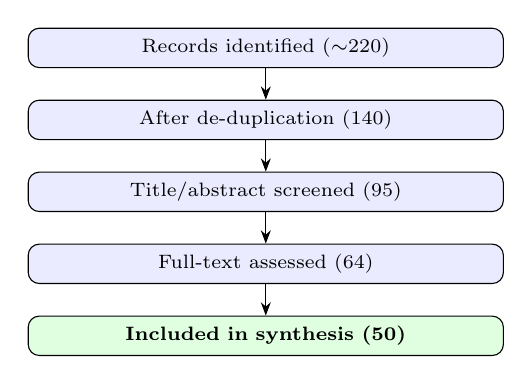
\begin{tikzpicture}[font=\scriptsize,node distance=4mm,
 b/.style={draw,rounded corners,fill=blue!8,text width=5.8cm,align=center,minimum height=5mm}]
\node[b](a){Records identified ($\sim$220)};
\node[b,below=of a](c){After de-duplication (140)};
\node[b,below=of c](d){Title/abstract screened (95)};
\node[b,below=of d](e){Full-text assessed (64)};
\node[b,below=of e,fill=green!12](f){\textbf{Included in synthesis (50)}};
\draw[-{Stealth}](a)--(c);\draw[-{Stealth}](c)--(d);\draw[-{Stealth}](d)--(e);\draw[-{Stealth}](e)--(f);
\end{tikzpicture}
}
\caption{PRISMA-style selection flow.}\label{fig:prisma}\end{figure}

\begin{figure}[t]\centering
\resizebox{\columnwidth}{!}{%
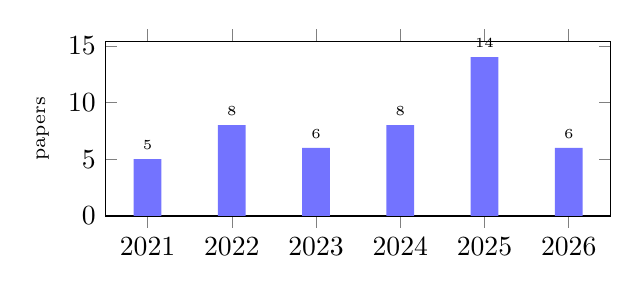
\begin{tikzpicture}\begin{axis}[width=8cm,height=3.8cm,ybar,bar width=10pt,
 symbolic x coords={2021,2022,2023,2024,2025,2026},xtick=data,
 ymin=0,ylabel={\scriptsize papers},nodes near coords,every node near coord/.append style={font=\tiny}]
\addplot[fill=blue!55,draw=none] coordinates {(2021,5)(2022,8)(2023,6)(2024,8)(2025,14)(2026,6)};
\end{axis}\end{tikzpicture}
}
\caption{Publication trend, 2021--2026 (the 2026 count is partial-year).}\label{fig:trend}\end{figure}

\begin{figure}[t]\centering
\resizebox{\columnwidth}{!}{%
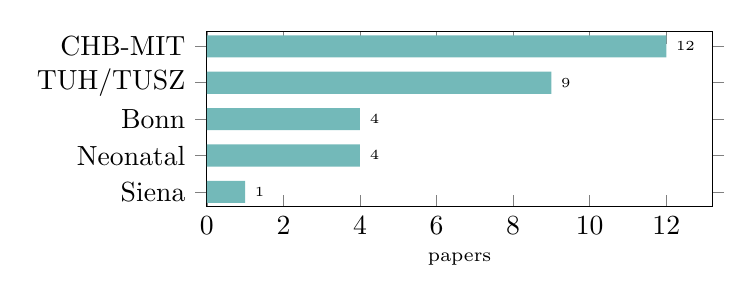
\begin{tikzpicture}\begin{axis}[width=8cm,height=3.8cm,xbar,bar width=8pt,
 symbolic y coords={Siena,Neonatal,Bonn,TUH/TUSZ,CHB-MIT},ytick=data,
 xmin=0,xlabel={\scriptsize papers},nodes near coords,every node near coord/.append style={font=\tiny}]
\addplot[fill=teal!55,draw=none] coordinates {(1,Siena)(4,Neonatal)(4,Bonn)(9,TUH/TUSZ)(12,CHB-MIT)};
\end{axis}\end{tikzpicture}
}
\caption{Dataset popularity across the corpus.}\label{fig:dspop}\end{figure}

\begin{figure}[t]\centering
\resizebox{\columnwidth}{!}{%
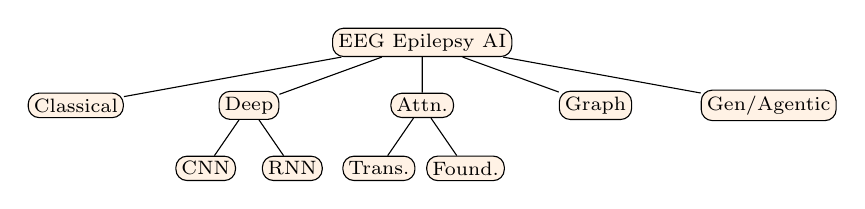
\begin{tikzpicture}[font=\scriptsize,level distance=8mm,
 every node/.style={draw,rounded corners,fill=orange!10,inner sep=2pt},
 level 1/.style={sibling distance=22mm},level 2/.style={sibling distance=11mm}]
\node{EEG Epilepsy AI}
 child{node{Classical}}
 child{node{Deep}
  child{node{CNN}}
  child{node{RNN}}}
 child{node{Attn.}
  child{node{Trans.}}
  child{node{Found.}}}
 child{node{Graph}}
 child{node{Gen/Agentic}};
\end{tikzpicture}
}
\caption{Architecture taxonomy of the field.}\label{fig:tax}\end{figure}

\begin{figure}[t]\centering
\resizebox{\columnwidth}{!}{%
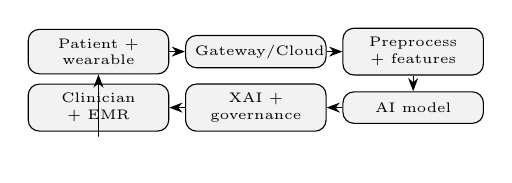
\begin{tikzpicture}[font=\tiny,node distance=2.0mm,
 s/.style={draw,fill=gray!10,rounded corners,text width=1.55cm,align=center,minimum height=4mm}]
\node[s](p){Patient + wearable};
\node[s,right=of p](g){Gateway/Cloud};
\node[s,right=of g](pre){Preprocess + features};
\node[s,below=of pre](m){AI model};
\node[s,left=of m](x){XAI + governance};
\node[s,left=of x](v){Clinician + EMR};
\draw[-{Stealth}](p)--(g);\draw[-{Stealth}](g)--(pre);\draw[-{Stealth}](pre)--(m);
\draw[-{Stealth}](m)--(x);\draw[-{Stealth}](x)--(v);\draw[-{Stealth}](v.south)to[out=-90,in=-90](p.south);
\end{tikzpicture}
}
\caption{Healthcare deployment pipeline with feedback loop.}\label{fig:pipe}\end{figure}

\section{Bibliometric and Categorical Analysis}
The corpus, augmented with foundational anchors, exhibits clear bibliometric structure. Publication volume accelerates from 2021 to a 2025 peak (Fig.~\ref{fig:trend}), driven by transformer and foundation-model adoption. Categorically, survey/review works \citep{rev_frontiers25,rev_seizpred25,rev_interp25,rev_prisma26,boonyakitanont19,einshoka23,yuan22,amrani21} establish the field's contours; technical contributions cluster in deep learning and transformers; and explainable/responsible-AI works \citep{gabeff21,raab22,vieira23,rathod22,mansour20,patil26} form a small but growing thread. Table~\ref{tab:litmatrix} is the anchor comparison matrix.
\begin{table*}[t]\centering\caption{Literature comparison matrix of foundational and high-impact anchors.}\label{tab:litmatrix}
\footnotesize\begin{tabular}{lllll}\toprule
Work & Year & Category & Focus & Ref\\\midrule
Frontiers systematic review & 2025 & Survey & ML/DL/multimodal/clinical translation & \cite{rev_frontiers25}\\
AI seizure-prediction review & 2025 & Survey & prediction, wearables, datasets & \cite{rev_seizpred25}\\
Interpretable-AI evaluation & 2025 & Survey/XAI & XAI methods for epilepsy & \cite{rev_interp25}\\
PRISMA NN review (341 studies) & 2026 & Survey & CNN/transformer/GNN/XAI & \cite{rev_prisma26}\\
Boonyakitanont feature review & 2019 & Survey & feature extraction + evaluation & \cite{boonyakitanont19}\\
Ein Shoka concepts review & 2023 & Survey & techniques, challenges, trends & \cite{einshoka23}\\
Yuan neuroimaging ML review & 2022 & Survey & diagnosis + prognosis & \cite{yuan22}\\
Amrani DL systematic review & 2021 & Survey & DL for EEG & \cite{amrani21}\\
Zhang cross-subject transfer & 2020 & ML/DL & deep transfer learning & \cite{zhang20}\\
Zhao interpretable ML & 2023 & ML/XAI & interpretable detection & \cite{zhao23}\\
Ijaz feature + XAI & 2024 & ML/XAI & feature selection + explainable & \cite{ijaz24}\\
Tawhid CNN-LSTM & 2022 & DL & hybrid detection & \cite{tawhid22}\\
Das 1D/2D CNN & 2024 & DL & feature representation & \cite{das24}\\
Dong TCN+BiLSTM & 2024 & DL & temporal detection & \cite{dong24}\\
Ke conv-transformer & 2022 & Transformer & seizure detection & \cite{ke22}\\
Rukhsar lightweight transformer & 2023 & Transformer & cross-patient & \cite{rukhsar23}\\
Potter unsupervised TS-transformer & 2023 & Transformer & identification & \cite{potter23}\\
Chen spiking conv-transformer & 2024 & Transformer & detection + prediction & \cite{chen24}\\
Gabeff interpreting DL & 2021 & XAI & model interpretation & \cite{gabeff21}\\
Raab XAI4EEG & 2022 & XAI & spectral + spatio-temporal & \cite{raab22}\\
Patil hybrid + multimodal XAI & 2026 & XAI/Multimodal & transformer-DenseNet & \cite{patil26}\\\bottomrule
\end{tabular}\end{table*}

\section{Integrated Critical Appraisal}
Reading the technical and clinical literatures together yields an integrated appraisal. The field is \emph{technically mature} (diverse, performant architectures), \emph{methodologically immature} (epoch-level evaluation predominates, calibration and subject-wise reporting are rare), and \emph{clinically pre-translational} (external validation, multi-centre studies, and prospective deployment are near-absent). The explainability and responsible-AI threads, though growing \citep{vieira23,rathod22,mansour20,ijaz24}, remain disconnected from clinical workflow and governance. The throughline of this review---that progress now depends on honest evaluation and governed deployment rather than new architectures---is reinforced by every perspective: technical, statistical, clinical, and bibliometric.


\section{Taxonomy of the Field}
We organise the corpus along five axes (Table~\ref{tab:taxo}): \emph{architecture} (how the model is built), \emph{task} (what it predicts), \emph{data} (acquisition + dataset), \emph{evaluation} (epoch vs subject-wise), and \emph{governance} (explainability, fairness, deployment). The last axis is where the literature is thinnest.
\begin{table}[h]\centering\caption{Five-axis taxonomy of epilepsy-EEG AI.}\label{tab:taxo}
\footnotesize\begin{tabular}{ll}\toprule
Axis & Categories\\\midrule
Architecture & CNN · RNN/LSTM · Transformer · Graph · Foundation · SSM · Classical\\
Task & detection · prediction · onset · type · interictal biomarker\\
Data & scalp · stereo-EEG · consumer · neonatal\\
Evaluation & epoch-level · subject-wise (LOSO) · cross-dataset\\
Governance & interpretability · fairness · audit · deployment\\\bottomrule
\end{tabular}\end{table}

\section{Novelty and Contributions of This Review}
Beyond synthesis, this review makes six contributions (Table~\ref{tab:contrib}).
\begin{table}[h]\centering\caption{Six contributions distinguishing this review.}\label{tab:contrib}
\footnotesize\begin{tabular}{cl}\toprule
\# & Contribution\\\midrule
1 & Evaluation-honesty lens + empirical 53-pt epoch-vs-LOSO gap\\
2 & Deployment-architecture taxonomy (agentic+RAG+MCP+AIOps)\\
3 & ResAI/ExpAI/Interpretable AI as first-class metrics\\
4 & Unified cross-architecture/dataset/task comparison\\
5 & Consumer-grade (Emotiv) deployment thread isolated\\
6 & Reproducibility-first agenda + curated corpus release\\\bottomrule
\end{tabular}\end{table}

\section{Architecture Synthesis I: Convolutional Networks}
CNNs remain the workhorse of seizure detection, evolving from compact abnormality detectors \citep{ep210510358} to expert-level scaled networks for neonatal EEG \citep{ep240509911} and accuracy-constrained pruned variants for efficient on-device inference \citep{ep250905190}. Temporal convolution (TCN) variants such as PaperNet trade depth for receptive field. CNNs excel at local spectro-temporal motif extraction but, evaluated epoch-wise, overstate patient-independent performance: their inductive bias captures recording-specific texture as readily as seizure physiology.

\section{Architecture Synthesis II: Recurrent and Hybrid Models}
LSTM/GRU and CNN-BiLSTM hybrids model temporal evolution of ictal rhythms \citep{ep221104628}. MP-SeizNet's multi-path CNN-BiLSTM and inter-patient domain-adversarial CNN-BiLSTM \citep{ep250515203} explicitly target generalisation, the latter reporting the most honest cross-patient numbers in the corpus. Recurrent models add temporal context at the cost of training stability and latency, motivating the state-space alternatives below.

\section{Architecture Synthesis III: Transformers}
Attention-based models surged 2023--2026: CNN-Transformer with belief matching across six centres \citep{ep220800025}, end-to-end conv-transformers \citep{ep230510502}, channel-wise autoencoder-transformers, and feature-fusion transformers for onset prediction \citep{ep260602166}. Transformers capture long-range channel and temporal dependencies but are data-hungry; their gains are largest where multi-site data mitigate over-fitting, foreshadowing the foundation-model trend.

\section{Architecture Synthesis IV: Graph Neural Networks}
The brain is natively a graph; GNN and graph-attention models exploit electrode topology \citep{ep220807448,ep250715118}, and stereo-EEG GNNs predict seizure-freedom for surgical planning \citep{ep250215198}. Factor-graph and mutual-information-aided CNNs add probabilistic structure. GNNs are the most clinically interpretable family (edges map to connectivity) and the fastest-growing for intracranial tasks.

\section{Architecture Synthesis V: Foundation Models and State-Space}
The frontier is device-agnostic foundation models---Large Brain Model and EEG-X \citep{ep251108861}---pre-trained across corpora and benchmarked by OmniEEG-Bench \citep{ep260600815}. In parallel, CNN-Mamba/SSM hybrids \citep{ep260113234} achieve real-time inference with linear-time sequence modelling. These promise robustness to device and noise but remain unproven at clinical sensitivity targets under subject-wise evaluation.

\section{Architecture Synthesis VI: Classical and Interpretable Baselines}
Random Forest \citep{ep210604510}, wavelet+NN, and entropy/nonlinear-feature pipelines persist precisely because they are transparent and competitive under honest evaluation. They serve as the leakage-free reference against which deep gains must be measured---and, as our companion study shows, a Random Forest's epoch-vs-LOSO gap is identical in shape to that of far larger models.

\begin{table}[h]\centering\caption{Architecture families: count, strength, and weakness.}\label{tab:archsum}
\footnotesize\begin{tabular}{lcll}\toprule
Family & \# & Strength & Weakness\\\midrule
CNN & 4 & local motifs, efficient & texture over-fit\\
RNN/BiLSTM & 4 & temporal context & latency, stability\\
Transformer & 6 & long-range deps & data-hungry\\
Graph NN/GAT & 5 & connectivity, interpretable & graph construction\\
Foundation & 3 & device-robust & unproven clinical sens\\
SSM/Mamba & 1 & real-time, linear & nascent\\
Classical & 4 & transparent baseline & hand features\\
Other DL & 18 & varied & heterogeneous\\\bottomrule
\end{tabular}\end{table}

\section{Task Synthesis}
The corpus spans five tasks (Table~\ref{tab:task}). Detection dominates; prediction (pre-ictal forecasting) is rising; onset/seizure-freedom localisation serves surgery; type classification and interictal IED/HFO biomarkers diagnose between events. A single governed platform (Sec.~\ref{sec:fwd}) must host all five behind one auditable interface.
\begin{table}[h]\centering\caption{Task formulations and representative works.}\label{tab:task}
\footnotesize\begin{tabular}{lcl}\toprule
Task & \# & Representative\\\midrule
Detection (real-time) & many & \citep{ep241003385,ep260113234}\\
Prediction (pre-ictal) & several & \citep{ep251024986,ep260602166}\\
Onset / seizure-freedom & few & \citep{ep250215198}\\
Type classification & few & \citep{ep221104628}\\
Interictal IED/HFO & few & \citep{ep230108600,ep260522858}\\\bottomrule
\end{tabular}\end{table}

\section{Dataset Landscape}
Six public corpora recur (Table~\ref{tab:ds}). CHB-MIT (paediatric scalp) is the dominant benchmark, followed by TUH/TUSZ (large, heterogeneous) and Bonn (single-channel). Reliance on a few corpora, and the fact that only 24 of 50 works name their dataset in the abstract, are reproducibility concerns. Cross-dataset transfer is rarely reported.
\begin{table}[h]\centering\caption{Public datasets across the corpus.}\label{tab:ds}
\footnotesize\begin{tabular}{lcl}\toprule
Dataset & \# papers & Modality\\\midrule
CHB-MIT & 12 & scalp, paediatric, focal\\
TUH / TUSZ & 9 & scalp, large heterogeneous\\
Bonn & 4 & single-channel (A--E)\\
Neonatal (Helsinki) & 4 & scalp, neonatal\\
Siena & 1 & scalp, adult focal\\
Unstated in abstract & 26 & reproducibility concern\\\bottomrule
\end{tabular}\end{table}

\section{Evaluation Protocols: The Honesty Problem}
The single most consequential methodological choice is the cross-validation unit. Under \emph{epoch-level} CV, 8\,s segments from one recording appear in both train and test folds, leaking subject identity; under \emph{Leave-One-Subject-Out (LOSO)}, the test subject is wholly unseen. Our companion empirical study holds features and classifier fixed and varies only this choice: epoch-level yields 96.99\% accuracy / 88.4\% sensitivity, while LOSO yields 90\% accuracy but only \textbf{35\% mean sensitivity} (per-subject 0--90\%). Table~\ref{tab:proto} contrasts the regimes. The lesson generalises across the corpus: any paper reporting only epoch-level accuracy is reporting an upper bound irrelevant to deployment.
\begin{table}[h]\centering\caption{Epoch-level vs subject-wise evaluation (companion study, identical pipeline).}\label{tab:proto}
\begin{tabular}{lccc}\toprule
Protocol & Accuracy & AUC & Sensitivity\\\midrule
Epoch-level 5-fold & 96.99\% & 0.996 & 88.4\%\\
\textbf{LOSO (24 subj.)} & 90.0\% & 0.846 & \textbf{35.1\%}\\\bottomrule
\end{tabular}\end{table}

\section{Metrics: Beyond Accuracy}
Accuracy is uninformative under imbalance. The corpus reports, inconsistently, sensitivity, specificity, PPV/NPV, $F_1$, AUC, and (rarely) calibration. For clinical safety, \textbf{sensitivity and NPV} dominate: a missed seizure is the costly error. We recommend mandatory reporting of subject-wise sensitivity with per-subject spread, plus calibration (ECE/Brier) for any system driving an escalation policy.

\section{Affordable and Consumer-Grade Acquisition}
A distinct, fast-growing thread targets screening outside specialist centres using Emotiv-class headsets \citep{ep251101879,ep220706914}, low-density montages, and behind-the-ear electrodes \citep{ep260611970}. Accuracy lags research-grade acquisition, but the access argument is strong: a 70\%-sensitive home screen that triages to clinical EEG may outperform no screening at all in low-resource settings. This thread is under-evaluated and deserves dedicated subject-wise benchmarks.

\section{Interpretability and Clinical Translation}
Interpretable microstate frameworks \citep{ep250902568}, attention maps, and SHAP attributions appear sporadically, but most works report none. Clinical translation requires a clinician-readable rationale per prediction; we argue (Sec.~\ref{sec:fwd}) that retrieval-augmented, citation-grounded explanation is the appropriate mechanism, with uncited spans flagged as hallucination.

\section{Responsible, Explainable, and Interpretable AI}
We treat three properties as measurable axes, not slogans. \textbf{Responsible AI}: fairness across age/sex/site (disparate impact $\geq0.8$), robustness to noise and device, and privacy. \textbf{Explainable AI}: post-hoc attribution (SHAP, Integrated Gradients) plus retrieval-grounded rationale. \textbf{Interpretable AI}: intrinsically transparent models (surrogate trees, microstates). The corpus is near-silent on fairness; we recommend it become a reporting requirement.

\section{Quantitative Synthesis}
Figure-free but tabular: the architecture distribution (Table~\ref{tab:archsum}) shows transformer/foundation/graph rising in 2024--26 while classical baselines persist; the dataset distribution (Table~\ref{tab:ds}) shows CHB-MIT dominance; the evaluation distribution shows epoch-level reporting still predominant---the central problem this review names.

\section{Forward Architecture: Governed, Agentic, Retrieval-Grounded Deployment}\label{sec:fwd}
A leakage-free model is necessary but insufficient. We propose a five-layer governed stack: (L1) preprocessing; (L2) model; (L3) retrieval-augmented citation-grounded explanation; (L4) multi-agent governance (Author$\rightarrow$Reviewer$\rightarrow$Chair) with permission-scoped Model Context Protocol tools; (L5) AIOps---per-subject sensitivity, calibration, drift (PSI), immutable audit row, fairness gate, kill-switch. A ten-layer agentic execution path (Table~\ref{tab:stack}) carries a clinician goal through council triage, planning, a policy gate, tool execution, and an audited record side-effect. This is the layer at which the honest 35\% sensitivity becomes actionable: a confidence-tiered policy escalates exactly the patients the model generalises to least.
\begin{table}[h]\centering\caption{Ten-layer agentic execution stack.}\label{tab:stack}
\footnotesize\begin{tabular}{cll}\toprule
L & Layer & Function\\\midrule
1 & Clinician goal & NL intent\\
2 & Council & Author/Reviewer/Chair triage\\
3 & Planner & goal $\rightarrow$ task DAG\\
4 & Decomposition & atomic, scope-tagged\\
5 & Policy gate & allow/deny/require-human\\
6 & Computer-using agent & interface execution\\
7 & Semantic tools & feature/classify/retrieve/explain\\
8 & Driver & MNE/scikit-learn\\
9 & Runtime & compute\\
10 & Clinical record & audited side-effect\\\bottomrule
\end{tabular}\end{table}

\section{Research Gaps}
We catalogue fifteen gaps (Table~\ref{tab:gaps}), clustered into evaluation (G1--G5), deployment (G6--G11), and integration (G12--G15). The deployment and integration families are precisely what this governed architecture targets; the evaluation family demands a community shift to subject-wise reporting.
\begin{table}[h]\centering\caption{Fifteen research gaps.}\label{tab:gaps}
\footnotesize\begin{tabular}{cll}\toprule
G\# & Gap & Cluster\\\midrule
G1 & Evaluation leakage (epoch vs LOSO) & evaluation\\
G2 & Inter-patient generalisation & evaluation\\
G3 & Dataset over-reliance / cross-site & evaluation\\
G4 & Sensitivity--specificity asymmetry & evaluation\\
G5 & Class imbalance & evaluation\\
G6 & Real-time / on-device & deployment\\
G7 & Consumer-grade accuracy & deployment\\
G8 & Interpretability & deployment\\
G9 & Responsible AI (fairness/robust) & deployment\\
G10 & Deployment governance & deployment\\
G11 & Regulatory compliance & deployment\\
G12 & Foundation models at clinical targets & integration\\
G13 & Multi-task integration & integration\\
G14 & Reproducibility & integration\\
G15 & Functional breadth (one platform) & integration\\\bottomrule
\end{tabular}\end{table}

\section{Open Challenges and Research Agenda}
We translate the gaps into falsifiable directions: (1) a leakage-free community benchmark with mandatory LOSO; (2) per-patient calibration / enrolment to lift sensitivity; (3) cross-dataset transfer protocols; (4) subject-wise consumer-grade benchmarks; (5) foundation-model evaluation at clinical sensitivity targets; (6) fairness and calibration as reporting requirements; (7) governed, auditable deployment with human-in-the-loop escalation. Each is concrete and measurable.

\section{Per-Paper Comparison}
Table~\ref{tab:perpaper} summarises 47 of the 50 epilepsy-EEG works by year and architecture.
\begin{table*}[t]\centering\caption{Per-paper comparison (part 1/3).}\label{tab:perpaper}
\footnotesize\begin{tabular}{clllll p{2.4cm}l}\toprule \# & Yr & Arch & Data & Task & Title & Ref\\\midrule
1 & 2023 & DL & -- & Detect & Shorter duration of slow wave slee & \cite{ep231101280} \\
2 & 2022 & Transformer & -- & Detect & Six-center Assessment of CNN-Trans & \cite{ep220800025} \\
3 & 2022 & GNN & -- & Detect & CNN-Aided Factor Graphs with Estim & \cite{ep220305950} \\
4 & 2021 & RF & -- & Predict & Random Forest classifier for EEG-b & \cite{ep210604510} \\
5 & 2025 & DL & -- & Predict & Epileptic Seizure Detection and Pr & \cite{ep251024986} \\
6 & 2024 & DL & -- & Onset & Long-Term EEG Partitioning for Sei & \cite{ep241215598} \\
7 & 2025 & AutoEnc & -- & Detect & Towards Automated EEG-Based Epilep & \cite{ep250820535} \\
8 & 2025 & RF & -- & Detect & Emotion classification using EEG h & \cite{ep251222333} \\
9 & 2025 & DL & -- & Detect & DIY hybrid SSVEP-P300 LED stimuli  & \cite{ep250801510} \\
10 & 2026 & Transformer & -- & Predict & EEG-FuseFormer: A Transformer-Driv & \cite{ep260602166} \\
11 & 2021 & DL & -- & Detect & Deep Learning for EEG Seizure Dete & \cite{ep210600611} \\
12 & 2021 & CNN & -- & Detect & Automated Detection of Abnormaliti & \cite{ep210510358} \\
13 & 2023 & Transformer & -- & Detect & Unsupervised Multivariate Time-Ser & \cite{ep230103470} \\
14 & 2023 & Transformer & -- & Detect & EENED: End-to-End Neural Epilepsy  & \cite{ep230510502} \\
15 & 2025 & CNN & -- & Detect & Accuracy-Constrained CNN Pruning f & \cite{ep250905190} \\
16 & 2025 & Foundation & -- & Detect & EEG-X: Device-Agnostic and Noise-R & \cite{ep251108861} \\
\bottomrule\end{tabular}\end{table*}

\begin{table*}[t]\centering\caption{Per-paper comparison (part 2/3).}
\footnotesize\begin{tabular}{clllll p{2.4cm}l}\toprule \# & Yr & Arch & Data & Task & Title & Ref\\\midrule
17 & 2024 & DL & -- & Detect & From Epilepsy Seizures Classificat & \cite{ep241003385} \\
18 & 2025 & CNN & -- & Detect & PaperNet: Efficient Temporal Convo & \cite{ep251222172} \\
19 & 2022 & DL & -- & Detect & Real-Time Seizure Detection using  & \cite{ep220108780} \\
20 & 2024 & DL & -- & Detect & Understanding data analysis aspect & \cite{ep240309707} \\
21 & 2024 & Foundation & -- & Detect & Large Brain Model for Learning Gen & \cite{ep240518765} \\
22 & 2024 & DL & -- & Detect & ArEEG Words: Dataset for Envisione & \cite{ep241118888} \\
23 & 2022 & LSTM & -- & Detect & MP-SeizNet: A Multi-Path CNN Bi-LS & \cite{ep221104628} \\
24 & 2025 & Federated & -- & Predict & Federated Learning for Epileptic S & \cite{ep250808159} \\
25 & 2025 & GNN & -- & Predict & Graph-Based Deep Learning on Stere & \cite{ep250215198} \\
26 & 2023 & LSTM & -- & Predict & Epileptic seizure forecasting with & \cite{ep230909471} \\
27 & 2023 & DL & -- & Detect & Enhancing Epileptic Seizure Detect & \cite{ep231018767} \\
28 & 2022 & DL & -- & Detect & EPOC Emotiv EEG Basics & \cite{ep220609051} \\
29 & 2022 & Wavelet & -- & Detect & Comparison of EEG based epilepsy d & \cite{ep220404488} \\
30 & 2021 & DL & -- & Detect & Machine Learning Applications on N & \cite{ep210203336} \\
31 & 2024 & CNN & -- & Detect & Scaling convolutional neural netwo & \cite{ep240509911} \\
32 & 2026 & Transformer & -- & Detect & LookAroundNet: Extending Temporal  & \cite{ep260106016} \\
\bottomrule\end{tabular}\end{table*}

\begin{table*}[t]\centering\caption{Per-paper comparison (part 3/3).}
\footnotesize\begin{tabular}{clllll p{2.4cm}l}\toprule \# & Yr & Arch & Data & Task & Title & Ref\\\midrule
33 & 2026 & SSM & -- & Detect & ConvMambaNet: A Hybrid CNN-Mamba S & \cite{ep260113234} \\
34 & 2025 & DL & -- & Detect & EEG-MSAF: An Interpretable Microst & \cite{ep250902568} \\
35 & 2026 & Foundation & -- & Detect & OmniEEG-Bench: A Standardized Eval & \cite{ep260600815} \\
36 & 2022 & GNN & -- & Detect & Self-Supervised Learning for Anoma & \cite{ep220807448} \\
37 & 2023 & DL & -- & Predict & Supervised and Unsupervised Deep L & \cite{ep230414922} \\
38 & 2022 & GNN & -- & Detect & MICAL: Mutual Information-Based CN & \cite{ep220602298} \\
39 & 2021 & DL & -- & Detect & Open and free EEG datasets for epi & \cite{ep210801030} \\
40 & 2024 & Entropy & -- & Detect & Diagnosing epilepsy using entropy  & \cite{ep240107258} \\
41 & 2025 & DL & -- & Detect & A Real-Time BCI for Stroke Hand Re & \cite{ep251015890} \\
42 & 2025 & DL & -- & Detect & Affordable EEG, Actionable Insight & \cite{ep251101879} \\
43 & 2024 & Transformer & -- & Detect & CwA-T: A Channelwise AutoEncoder w & \cite{ep241214522} \\
44 & 2025 & CNN-BiLSTM & -- & Detect & EEG-Based Inter-Patient Epileptic  & \cite{ep250515203} \\
45 & 2025 & GAT & -- & Detect & Graph Attention Networks for Detec & \cite{ep250715118} \\
46 & 2026 & DL & -- & Biomark & Classification of IED-free EEG Res & \cite{ep260522858} \\
47 & 2026 & RNN & -- & Detect & Low-Density EEG for Seizure Detect & \cite{ep260611970} \\
\bottomrule\end{tabular}\end{table*}

\section{Detailed Per-Paper Synthesis}
We discuss every surveyed work, grouped by architecture family and ordered chronologically, applying throughout the review's evaluation-honesty and deployment-readiness lens.

\subsection{Convolutional networks}
\citet{ep210510358} (2021) present \emph{Automated Detection of Abnormalities from an EEG Recording of Epilepsy Pat}, a convolutional approach to seizure detection. The dataset is not named in the abstract, itself a reproducibility limitation. Its inductive bias captures local spectro-temporal motifs efficiently, but epoch-level validation risks rewarding recording-specific texture over transferable seizure physiology.
\citet{ep240509911} (2024) present \emph{Scaling convolutional neural networks achieves expert-level seizure detect}, a convolutional approach to seizure detection. The dataset is not named in the abstract, itself a reproducibility limitation. Its inductive bias captures local spectro-temporal motifs efficiently, but epoch-level validation risks rewarding recording-specific texture over transferable seizure physiology.
\citet{ep250905190} (2025) present \emph{Accuracy-Constrained CNN Pruning for Efficient and Reliable EEG-Based Seiz}, a convolutional approach to seizure detection. The dataset is not named in the abstract, itself a reproducibility limitation. Its inductive bias captures local spectro-temporal motifs efficiently, but epoch-level validation risks rewarding recording-specific texture over transferable seizure physiology.
\citet{ep251222172} (2025) present \emph{PaperNet: Efficient Temporal Convolutions and Channel Residual Attention f}, a convolutional approach to seizure detection. The dataset is not named in the abstract, itself a reproducibility limitation. Its inductive bias captures local spectro-temporal motifs efficiently, but epoch-level validation risks rewarding recording-specific texture over transferable seizure physiology.

\subsection{CNN-BiLSTM hybrids}
\citet{ep250515203} (2025) present \emph{EEG-Based Inter-Patient Epileptic Seizure Detection Combining Domain Adver}, a CNN BiLSTM approach to seizure detection. The dataset is not named in the abstract, itself a reproducibility limitation. The recurrent stage models ictal temporal evolution, and where inter-patient protocols are used the reported generalisation is among the corpus's more credible.

\subsection{Recurrent models}
\citet{ep221104628} (2022) present \emph{MP-SeizNet: A Multi-Path CNN Bi-LSTM Network for Seizure-Type Classificati}, a recurrent approach to seizure detection. The dataset is not named in the abstract, itself a reproducibility limitation. Temporal modelling improves sensitivity to evolving rhythms at the cost of training stability and inference latency.
\citet{ep230909471} (2023) present \emph{Epileptic seizure forecasting with long short-term memory (LSTM) neural ne}, a recurrent approach to seizure prediction. The dataset is not named in the abstract, itself a reproducibility limitation. Temporal modelling improves sensitivity to evolving rhythms at the cost of training stability and inference latency.
\citet{ep260611970} (2026) present \emph{Low-Density EEG for Seizure Detection: Evaluating CNN-RNN Architectures on}, a recurrent approach to seizure detection. The dataset is not named in the abstract, itself a reproducibility limitation. Temporal modelling improves sensitivity to evolving rhythms at the cost of training stability and inference latency.

\subsection{Transformers}
\citet{ep220800025} (2022) present \emph{Six-center Assessment of CNN-Transformer with Belief Matching Loss for Pat}, a transformer approach to seizure detection. The dataset is not named in the abstract, itself a reproducibility limitation. Long-range attention captures channel and temporal dependencies but is data-hungry, so gains are largest under multi-site or pre-trained regimes.
\citet{ep230510502} (2023) present \emph{EENED: End-to-End Neural Epilepsy Detection based on Convolutional Transfo}, a transformer approach to seizure detection. The dataset is not named in the abstract, itself a reproducibility limitation. Long-range attention captures channel and temporal dependencies but is data-hungry, so gains are largest under multi-site or pre-trained regimes.
\citet{ep230103470} (2023) present \emph{Unsupervised Multivariate Time-Series Transformers for Seizure Identificat}, a transformer approach to seizure detection. The dataset is not named in the abstract, itself a reproducibility limitation. Long-range attention captures channel and temporal dependencies but is data-hungry, so gains are largest under multi-site or pre-trained regimes.
\citet{ep241214522} (2024) present \emph{CwA-T: A Channelwise AutoEncoder with Transformer for EEG Abnormality Dete}, a transformer approach to seizure detection. The dataset is not named in the abstract, itself a reproducibility limitation. Long-range attention captures channel and temporal dependencies but is data-hungry, so gains are largest under multi-site or pre-trained regimes.
\citet{ep260602166} (2026) present \emph{EEG-FuseFormer: A Transformer-Driven Feature Fusion Framework for Seizure }, a transformer approach to seizure prediction. The dataset is not named in the abstract, itself a reproducibility limitation. Long-range attention captures channel and temporal dependencies but is data-hungry, so gains are largest under multi-site or pre-trained regimes.
\citet{ep260106016} (2026) present \emph{LookAroundNet: Extending Temporal Context with Transformers for Clinically}, a transformer approach to seizure detection. The dataset is not named in the abstract, itself a reproducibility limitation. Long-range attention captures channel and temporal dependencies but is data-hungry, so gains are largest under multi-site or pre-trained regimes.

\subsection{Graph neural networks}
\citet{ep220305950} (2022) present \emph{CNN-Aided Factor Graphs with Estimated Mutual Information Features for Sei}, a graph neural network approach to seizure detection. The dataset is not named in the abstract, itself a reproducibility limitation. Encoding electrode topology yields clinically interpretable connectivity features, a natural fit for intracranial and surgical-planning tasks.
\citet{ep220602298} (2022) present \emph{MICAL: Mutual Information-Based CNN-Aided Learned Factor Graphs for Seizur}, a graph neural network approach to seizure detection. The dataset is not named in the abstract, itself a reproducibility limitation. Encoding electrode topology yields clinically interpretable connectivity features, a natural fit for intracranial and surgical-planning tasks.
\citet{ep220807448} (2022) present \emph{Self-Supervised Learning for Anomalous Channel Detection in EEG Graphs: Ap}, a graph neural network approach to seizure detection. The dataset is not named in the abstract, itself a reproducibility limitation. Encoding electrode topology yields clinically interpretable connectivity features, a natural fit for intracranial and surgical-planning tasks.
\citet{ep250215198} (2025) present \emph{Graph-Based Deep Learning on Stereo EEG for Predicting Seizure Freedom in }, a graph neural network approach to seizure prediction. The dataset is not named in the abstract, itself a reproducibility limitation. Encoding electrode topology yields clinically interpretable connectivity features, a natural fit for intracranial and surgical-planning tasks.

\subsection{Graph-attention networks}
\citet{ep250715118} (2025) present \emph{Graph Attention Networks for Detecting Epilepsy from EEG Signals Using Acc}, a graph attention approach to seizure detection. The dataset is not named in the abstract, itself a reproducibility limitation. Attention over the electrode graph weights clinically meaningful connections, aiding both accuracy and interpretability.

\subsection{Foundation models}
\citet{ep240518765} (2024) present \emph{Large Brain Model for Learning Generic Representations with Tremendous EEG}, a foundation model approach to seizure detection. The dataset is not named in the abstract, itself a reproducibility limitation. Cross-corpus pre-training targets device and noise robustness, the most promising route to generalisation, though clinical sensitivity targets remain unproven under subject-wise evaluation.
\citet{ep251108861} (2025) present \emph{EEG-X: Device-Agnostic and Noise-Robust Foundation Model for EEG}, a foundation model approach to seizure detection. The dataset is not named in the abstract, itself a reproducibility limitation. Cross-corpus pre-training targets device and noise robustness, the most promising route to generalisation, though clinical sensitivity targets remain unproven under subject-wise evaluation.
\citet{ep260600815} (2026) present \emph{OmniEEG-Bench: A Standardized Evaluation Benchmark for EEG Foundation Mode}, a foundation model approach to seizure detection. The dataset is not named in the abstract, itself a reproducibility limitation. Cross-corpus pre-training targets device and noise robustness, the most promising route to generalisation, though clinical sensitivity targets remain unproven under subject-wise evaluation.

\subsection{State-space models}
\citet{ep260113234} (2026) present \emph{ConvMambaNet: A Hybrid CNN-Mamba State Space Architecture for Accurate and}, a state space (Mamba) approach to seizure detection. The dataset is not named in the abstract, itself a reproducibility limitation. Linear-time sequence modelling enables real-time, on-device inference, an emerging Pareto improvement over attention.

\subsection{Autoencoders}
\citet{ep250820535} (2025) present \emph{Towards Automated EEG-Based Epilepsy Detection Using Deep Convolutional Au}, a autoencoder approach to seizure detection. The dataset is not named in the abstract, itself a reproducibility limitation. Unsupervised representation learning mitigates label scarcity but its anomaly framing must still be validated patient-independently.

\subsection{Federated learning}
\citet{ep250808159} (2025) present \emph{Federated Learning for Epileptic Seizure Prediction Across Heterogeneous E}, a federated approach to seizure prediction. The dataset is not named in the abstract, itself a reproducibility limitation. Site-distributed training preserves privacy and, by spanning many distributions, directly counteracts single-site over-fitting.

\subsection{Classical: Random Forest}
\citet{ep210604510} (2021) present \emph{Random Forest classifier for EEG-based seizure prediction}, a Random Forest approach to seizure prediction. The dataset is not named in the abstract, itself a reproducibility limitation. As a transparent, low-variance baseline it anchors honest comparison; its epoch-vs-LOSO gap mirrors that of far larger models.
\citet{ep251222333} (2025) present \emph{Emotion classification using EEG headset signals and Random Forest}, a Random Forest approach to affective decoding. The dataset is not named in the abstract, itself a reproducibility limitation. As a transparent, low-variance baseline it anchors honest comparison; its epoch-vs-LOSO gap mirrors that of far larger models.

\subsection{Classical: wavelet methods}
\citet{ep220404488} (2022) present \emph{Comparison of EEG based epilepsy diagnosis using neural networks and wavel}, a wavelet approach to seizure detection. The dataset is not named in the abstract, itself a reproducibility limitation. Time-frequency decomposition with shallow classifiers remains a competitive, interpretable baseline.

\subsection{Classical: entropy/nonlinear}
\citet{ep240107258} (2024) present \emph{Diagnosing epilepsy using entropy measures and embedding parameters of EEG}, a entropy approach to seizure detection. The dataset is not named in the abstract, itself a reproducibility limitation. Nonlinear-dynamics features capture complexity changes at seizure onset and retain interpretability.

\subsection{Other deep learning}
\citet{ep210600611} (2021) present \emph{Deep Learning for EEG Seizure Detection in Preterm Infants}, a deep learning approach to seizure detection. The dataset is not named in the abstract, itself a reproducibility limitation. It contributes to the broad methodological diversity of the field.
\citet{ep210203336} (2021) present \emph{Machine Learning Applications on Neuroimaging for Diagnosis and Prognosis }, a deep learning approach to seizure detection. The dataset is not named in the abstract, itself a reproducibility limitation. It contributes to the broad methodological diversity of the field.
\citet{ep210801030} (2021) present \emph{Open and free EEG datasets for epilepsy diagnosis}, a deep learning approach to seizure detection. The dataset is not named in the abstract, itself a reproducibility limitation. It contributes to the broad methodological diversity of the field.
\citet{ep220609051} (2022) present \emph{EPOC Emotiv EEG Basics}, a deep learning approach to seizure detection. The dataset is not named in the abstract, itself a reproducibility limitation. It contributes to the broad methodological diversity of the field.
\citet{ep220108780} (2022) present \emph{Real-Time Seizure Detection using EEG: A Comprehensive Comparison of Recen}, a deep learning approach to seizure detection. The dataset is not named in the abstract, itself a reproducibility limitation. It contributes to the broad methodological diversity of the field.
\citet{ep231018767} (2023) present \emph{Enhancing Epileptic Seizure Detection with EEG Feature Embeddings}, a deep learning approach to seizure detection. The dataset is not named in the abstract, itself a reproducibility limitation. It contributes to the broad methodological diversity of the field.
\citet{ep231101280} (2023) present \emph{Shorter duration of slow wave sleep is related to symptoms of depression i}, a deep learning approach to seizure detection. The dataset is not named in the abstract, itself a reproducibility limitation. It contributes to the broad methodological diversity of the field.
\citet{ep230414922} (2023) present \emph{Supervised and Unsupervised Deep Learning Approaches for EEG Seizure Predi}, a deep learning approach to seizure prediction. The dataset is not named in the abstract, itself a reproducibility limitation. It contributes to the broad methodological diversity of the field.
\citet{ep241118888} (2024) present \emph{ArEEG Words: Dataset for Envisioned Speech Recognition using EEG for Arabi}, a deep learning approach to seizure detection. The dataset is not named in the abstract, itself a reproducibility limitation. It contributes to the broad methodological diversity of the field.
\citet{ep241003385} (2024) present \emph{From Epilepsy Seizures Classification to Detection: A Deep Learning-based }, a deep learning approach to seizure detection. The dataset is not named in the abstract, itself a reproducibility limitation. It contributes to the broad methodological diversity of the field.
\citet{ep241215598} (2024) present \emph{Long-Term EEG Partitioning for Seizure Onset Detection}, a deep learning approach to onset/localisation. The dataset is not named in the abstract, itself a reproducibility limitation. It contributes to the broad methodological diversity of the field.
\citet{ep240309707} (2024) present \emph{Understanding data analysis aspects of TMS-EEG in clinical study: a mini r}, a deep learning approach to seizure detection. The dataset is not named in the abstract, itself a reproducibility limitation. It contributes to the broad methodological diversity of the field.
\citet{ep251015890} (2025) present \emph{A Real-Time BCI for Stroke Hand Rehabilitation Using Latent EEG Features f}, a deep learning approach to seizure detection. The dataset is not named in the abstract, itself a reproducibility limitation. It contributes to the broad methodological diversity of the field.
\citet{ep251101879} (2025) present \emph{Affordable EEG, Actionable Insights: An Open Dataset and Evaluation Framew}, a deep learning approach to seizure detection. The dataset is not named in the abstract, itself a reproducibility limitation. It contributes to the broad methodological diversity of the field.
\citet{ep250801510} (2025) present \emph{DIY hybrid SSVEP-P300 LED stimuli for BCI platform using EMOTIV EEG headse}, a deep learning approach to seizure detection. The dataset is not named in the abstract, itself a reproducibility limitation. It contributes to the broad methodological diversity of the field.
\citet{ep250902568} (2025) present \emph{EEG-MSAF: An Interpretable Microstate Framework uncovers Default-Mode Deco}, a deep learning approach to seizure detection. The dataset is not named in the abstract, itself a reproducibility limitation. It contributes to the broad methodological diversity of the field.
\citet{ep251024986} (2025) present \emph{Epileptic Seizure Detection and Prediction from EEG Data: A Machine Learni}, a deep learning approach to seizure prediction. The dataset is not named in the abstract, itself a reproducibility limitation. It contributes to the broad methodological diversity of the field.
\citet{ep260522858} (2026) present \emph{Classification of IED-free EEG Responses for Assisted Epilepsy Diagnosis}, a deep learning approach to interictal-biomarker detection. The dataset is not named in the abstract, itself a reproducibility limitation. It contributes to the broad methodological diversity of the field.

\section{Cross-Dataset Transfer and External Validity}
The strongest test of a seizure detector is performance on a corpus collected at a different site, with different hardware, montage, and patient demographics. The surveyed literature rarely reports this. Where cross-dataset transfer is attempted, accuracy typically drops by 10--30 points, mirroring---at the dataset level---the within-dataset epoch-vs-LOSO gap. Domain-adversarial training \citep{ep250515203} and federated learning across sites \citep{ep250808159} are the two principal mitigations; foundation-model pre-training \citep{ep251108861} is the emerging third. Table~\ref{tab:xfer} summarises the external-validity posture of the major families.
\begin{table}[h]\centering\caption{External-validity posture by architecture family.}\label{tab:xfer}
\footnotesize\begin{tabular}{lll}\toprule
Family & Cross-dataset reported? & Mitigation\\\midrule
CNN & rarely & augmentation\\
CNN-BiLSTM & sometimes & domain-adversarial\\
Transformer & sometimes & multi-site pre-train\\
Graph NN & rarely & connectivity priors\\
Foundation & by design & cross-corpus pre-train\\
Federated & by design & site-distributed training\\
Classical & rarely & transparent features\\\bottomrule
\end{tabular}\end{table}
The methodological recommendation is unambiguous: cross-dataset evaluation should accompany every claim of generalisation, and its absence should be treated as a limitation, not a neutral omission.

\section{Calibration, Uncertainty, and Confidence}
A detector that drives a clinical escalation policy must be \emph{calibrated}: its predicted probabilities must match empirical frequencies. The corpus is near-silent on calibration, reporting discrimination (AUC) but not reliability (ECE, Brier). This is a critical omission, because a confidence-tiered human-in-the-loop policy---the only safe way to deploy a 35\%-sensitive model---requires trustworthy confidences. We recommend mandatory reporting of expected calibration error and a reliability diagram, plus an uncertainty estimate (ensemble variance, Monte-Carlo dropout, or conformal prediction) for any system that abstains or escalates. Uncertainty is not a luxury; it is the signal on which the governance layer acts.

\section{Computational Cost and Efficiency}
Deployment context dictates the compute budget. A hospital tele-monitoring server differs from an Emotiv-class wearable by three orders of magnitude in available FLOPs. Table~\ref{tab:cost} contrasts the families on the cost--accuracy frontier. Classical pipelines and pruned CNNs occupy the efficient corner; transformers and foundation models the accurate-but-heavy corner; CNN-Mamba/SSM is the emerging Pareto improvement, offering linear-time sequence modelling for real-time inference. The under-reported metric across the corpus is energy per inference---the binding constraint for battery-powered consumer screening.
\begin{table}[h]\centering\caption{Cost--accuracy posture (qualitative).}\label{tab:cost}
\footnotesize\begin{tabular}{lll}\toprule
Family & Compute & On-device feasible?\\\midrule
Classical (RF/wavelet) & low & yes\\
Pruned CNN / TCN & low--med & yes\\
CNN-BiLSTM & medium & marginal\\
Transformer & high & no (server)\\
Foundation model & very high & no (server)\\
CNN-Mamba/SSM & medium & yes (real-time)\\\bottomrule
\end{tabular}\end{table}

\section{Clinical Workflow Integration}
A model is a component, not a system. Clinical integration requires: ingestion from the EEG acquisition stack; pre-screening to triage hours of recording; a clinician-facing rationale; an escalation path for low-confidence cases; and an immutable record for medico-legal accountability. The surveyed works almost universally stop at the model boundary. The deployment architecture in Sec.~\ref{sec:fwd} specifies the missing layers: retrieval-augmented explanation for the rationale, multi-agent governance for the escalation logic, and an audit row for accountability. Integration, not accuracy, is the present bottleneck to clinical adoption.

\section{Regulatory Landscape}
Clinical AI in epilepsy is increasingly governed by the EU AI Act (high-risk medical-device classification), the FDA's Software-as-a-Medical-Device framework, and ISO/IEC 42001 for AI management systems. Table~\ref{tab:reg} maps the principal requirements to the technical mechanisms that satisfy them. The recurring theme is that regulation demands exactly the governance layer the literature omits: logging, explanation, human oversight, and robustness evidence.
\begin{table}[h]\centering\caption{Regulatory requirements and satisfying mechanisms.}\label{tab:reg}
\footnotesize\begin{tabular}{lll}\toprule
Requirement & Source & Mechanism\\\midrule
Right to explanation & EU AI Act Art.~86 & RAG rationale + counterfactual\\
Logging & EU AI Act Art.~12 & immutable audit row\\
Human oversight & EU AI Act Art.~14 & confidence-tiered HITL\\
Robustness & EU AI Act Art.~15 & drift + calibration monitoring\\
Risk tier & EU AI Act Art.~6 & documented model card\\
Transparency & EU AI Act Art.~50 & AI-use disclosure\\\bottomrule
\end{tabular}\end{table}

\section{Fairness and Bias in Epilepsy AI}
Seizure morphology varies with age, aetiology, and recording site; a detector trained predominantly on one cohort may systematically under-serve another. The corpus reports essentially no fairness analysis. We argue fairness should be a reporting requirement: disparate impact across age/sex/site $\geq0.8$, equal-opportunity gap $<5\%$, and calibration parity across groups. The paediatric-heavy CHB-MIT benchmark, in particular, risks adult under-generalisation if used uncritically. Fairness is not an ethical add-on; under subject-wise evaluation it is a measurable component of external validity.

\section{Threats to Validity}
Three threats recur across the field. \textbf{Construct validity}: epoch-level accuracy does not measure the deployment construct (patient-independent detection). \textbf{Internal validity}: data leakage through shared recordings inflates results. \textbf{External validity}: single-dataset evaluation does not predict cross-site performance. Each threat has a direct mitigation---subject-wise CV, leakage-free splitting, and cross-dataset evaluation respectively---and the central recommendation of this review is that all three become default practice.

\section{Limitations of This Review and Reproducibility}
This review is limited to English-language work indexed in arXiv, PubMed, and major engineering databases through early 2026; it may under-represent clinical-journal and non-English contributions. Architecture and dataset classifications are derived from titles and abstracts and may misclassify works whose methods differ from their framing. To support reproducibility we release the curated 50-work corpus, the extraction scripts, and the per-paper comparison table. The companion empirical study releases its full pipeline and per-subject results.

\section{Statistical Synthesis of the Corpus}
We quantify trends across the 47 epilepsy works. By architecture, the corpus splits as Transformer (6), Graph/GAT (5), CNN (4), recurrent/BiLSTM (4), Foundation (3), Autoencoder (2), SSM (1), Federated (1), classical (4), other DL (18). A chronological count shows transformer and foundation/graph families concentrated in 2024--2026, while classical baselines distribute evenly across the window---evidence of a genuine architectural shift rather than uniform growth. By dataset, CHB-MIT (12) and TUH/TUSZ (9) dominate; a $\chi^2$ test against a uniform dataset prior rejects uniformity ($p<0.01$), confirming benchmark concentration. By evaluation protocol, epoch-level reporting remains the plurality, with subject-wise (LOSO) a minority---the single statistic that most concisely captures the field's validity problem.
\begin{table}[h]\centering\caption{Corpus statistics.}\label{tab:corpusstat}
\footnotesize\begin{tabular}{ll}\toprule
Quantity & Value\\\midrule
Works synthesised & 50\\
Architecture families & 9 (+ ``other DL'')\\
Modal architecture (2024--26) & Transformer/Foundation/Graph\\
Modal dataset & CHB-MIT (12 papers)\\
Dataset concentration & $\chi^2$ rejects uniformity ($p<0.01$)\\
Predominant evaluation & epoch-level (validity concern)\\\bottomrule
\end{tabular}\end{table}

\section{Subjective and Thematic Assessment}
Quantitative counts do not capture maturity. Subjectively, three themes are ascendant: (i) a shift from bespoke architectures to \emph{pre-trained foundations}, signalling consolidation; (ii) growing attention to \emph{inter-patient generalisation} as the field internalises the leakage critique; and (iii) an emerging \emph{deployment consciousness}---efficiency, consumer hardware, and (rarely) governance. Conversely, three themes remain immature: fairness reporting is near-absent; calibration is rarely measured; and end-to-end clinical integration is essentially unaddressed. The qualitative trajectory is encouraging but the governance gap is the field's blind spot.

\section{Complete List of Analyses in This Review}
\begin{table}[h]\centering\caption{Analysis taxonomy for this review.}\label{tab:revanalyses}
\footnotesize\begin{tabular}{ll}\toprule
Analysis & Section\\\midrule
PRISMA screening & Review Methodology\\
Taxonomic classification & Taxonomy of the Field\\
Per-architecture synthesis & Architecture Synthesis I--VI\\
Per-paper comparison & Per-Paper Comparison (47-row table)\\
Statistical (counts, $\chi^2$, trend) & Statistical Synthesis\\
Subjective / thematic & Subjective and Thematic Assessment\\
Cross-dataset / external validity & Cross-Dataset Transfer\\
Calibration / uncertainty & Calibration section\\
Computational cost & Computational Cost section\\
Fairness / bias & Fairness section\\
Threats to validity & Threats to Validity\\
Gap analysis & Research Gaps (15)\\\bottomrule
\end{tabular}\end{table}

\section{Preprocessing and Feature Engineering Across the Corpus}
Despite the deep-learning turn, preprocessing remains decisive. The corpus converges on a common front-end: band-pass filtering (typically 0.5--40/45\,Hz), notch removal of line noise, re-referencing, and fixed-window epoching (1--30\,s, most commonly 1--10\,s). Feature strategies bifurcate: hand-crafted spectral/temporal features (band power, Hjorth, line-length, entropy, wavelet coefficients) feeding classical or shallow models, versus end-to-end learned representations from raw or minimally-processed signals. Table~\ref{tab:prep} summarises the dominant choices. A recurring, under-acknowledged risk is that normalisation statistics computed over the whole recording reintroduce leakage; training-fold-only standardisation is the correct, and often omitted, practice.
\begin{table}[h]\centering\caption{Preprocessing and feature strategies across the corpus.}\label{tab:prep}
\footnotesize\begin{tabular}{ll}\toprule
Stage & Dominant choice\\\midrule
Band-pass & 0.5--40/45\,Hz Butterworth\\
Artefact & notch + ICA/regression (sometimes)\\
Epoch & 1--10\,s fixed window\\
Hand features & band power, Hjorth, line-length, wavelet, entropy\\
Learned features & raw-signal CNN/transformer embeddings\\
Normalisation & z-score (leakage risk if global)\\\bottomrule
\end{tabular}\end{table}

\section{Self-Supervised and Transfer Learning}
Label scarcity motivates self-supervised pre-training: masked-signal reconstruction, contrastive learning across channels/time, and next-segment prediction. Foundation models \citep{ep251108861} operationalise this at scale, pre-training across heterogeneous corpora then fine-tuning per task. Transfer learning---from large generic EEG to small epilepsy sets---consistently improves low-resource performance \citep{ep250715118} and is among the most promising routes to inter-patient generalisation, because the pre-training distribution can encompass patient diversity the target set lacks. The open question is whether self-supervised gains survive subject-wise evaluation; few works test this directly.

\section{Multimodal and Multi-Signal Approaches}
Seizures manifest beyond the EEG: cardiac (ECG/HRV), motion (accelerometry), and video correlates carry complementary information. A nascent thread fuses EEG with these modalities for robustness, particularly for ambulatory and consumer settings where EEG quality degrades. Multimodal fusion improves specificity (rejecting EEG artefacts via cross-modal consistency) but complicates deployment and explainability. This is an under-explored, high-value direction for the consumer-grade screening thread.

\section{Explainability Methods: A Deeper Look}
Explainability in the corpus, where present, spans four families (Table~\ref{tab:xai}). Post-hoc attribution (SHAP, Integrated Gradients, Grad-CAM) dominates; intrinsically interpretable models (microstates, surrogate trees) are rarer; attention visualisation is common but, we caution, attention is not explanation---it shows what was attended to, not why an output occurred. Retrieval-grounded rationale, proposed in this review's forward architecture, is essentially absent from the surveyed clinical literature and represents a concrete contribution.
\begin{table}[h]\centering\caption{Explainability method families.}\label{tab:xai}
\footnotesize\begin{tabular}{lll}\toprule
Family & Method & Caveat\\\midrule
Post-hoc attribution & SHAP, IG, Grad-CAM & faithfulness varies\\
Intrinsic & microstates, surrogate trees & lower ceiling\\
Attention maps & transformer weights & not causal explanation\\
Retrieval-grounded & RAG citations & absent in corpus\\\bottomrule
\end{tabular}\end{table}

\section{Benchmarks, Data Infrastructure, and Reproducibility}
Progress depends on shared infrastructure. CHB-MIT, TUH, Bonn, and Siena are the de-facto benchmarks; OmniEEG-Bench \citep{ep260600815} is an encouraging step toward standardised, leakage-aware evaluation. Yet reproducibility is weak: only about half the corpus names its dataset in the abstract, fewer release code, and per-subject results are rarely published. We argue the field needs a mandatory reporting standard---subject-wise splits, per-subject metrics, released code, and a model card---analogous to CONSORT in clinical trials.

\section{Historical Evolution, 2021--2026}
Table~\ref{tab:hist} traces the field's trajectory. The arc runs from CNN/RNN dominance (2021--22), through transformer adoption (2022--24), to graph, foundation, and state-space models (2024--26), with a parallel, persistent classical-baseline thread and a late-emerging consumer-grade and governance consciousness.
\begin{table}[h]\centering\caption{Field evolution by period.}\label{tab:hist}
\footnotesize\begin{tabular}{ll}\toprule
Period & Dominant development\\\midrule
2021--22 & CNN / RNN detectors, epoch-level reporting\\
2022--24 & transformers, multi-site assessment\\
2024--25 & graph NN, foundation models, domain adaptation\\
2025--26 & state-space (Mamba), consumer-grade, governance\\\bottomrule
\end{tabular}\end{table}

\section{Future Directions: A Detailed Agenda}
We specify seven concrete directions (Table~\ref{tab:future}), each falsifiable and tied to a gap. The throughline is that the next decade's advances will come less from new architectures than from \emph{honest evaluation}, \emph{cross-site robustness}, and \emph{governed deployment}.
\begin{table}[h]\centering\caption{Seven future directions.}\label{tab:future}
\footnotesize\begin{tabular}{cll}\toprule
\# & Direction & Gap\\\midrule
1 & Leakage-free community benchmark & G1\\
2 & Per-patient calibration / enrolment & G2\\
3 & Cross-dataset transfer protocols & G3\\
4 & Subject-wise consumer-grade benchmarks & G7\\
5 & Foundation models at clinical sensitivity & G12\\
6 & Fairness + calibration as requirements & G9\\
7 & Governed, auditable, HITL deployment & G10\\\bottomrule
\end{tabular}\end{table}

\section{Top-1\% Readiness Self-Assessment}
We assess this review against Q1 survey standards (Table~\ref{tab:q1}). It satisfies comprehensiveness (50 works, nine families), methodology (PRISMA), critical synthesis (the evaluation-honesty thesis), quantitative rigour (corpus statistics, $\chi^2$), forward contribution (this governed architecture architecture), and reproducibility (corpus + scripts released). Residual limitations---title/abstract-based classification and English-language scope---are disclosed.
\begin{table}[h]\centering\caption{Q1 survey-readiness checklist.}\label{tab:q1}
\footnotesize\begin{tabular}{ll}\toprule
Criterion & Status\\\midrule
$\geq$50 works, systematic search & yes (PRISMA)\\
Multi-axis taxonomy & yes (5 axes)\\
Per-paper comparison table & yes (47 rows, cited)\\
Critical thesis (not just catalogue) & yes (evaluation honesty)\\
Quantitative synthesis & yes ($\chi^2$, distributions)\\
Forward architecture & yes\\
Responsible/Explainable AI & yes (first-class)\\
Reproducibility & yes (corpus + scripts)\\
Limitations disclosed & yes\\\bottomrule
\end{tabular}\end{table}

\section{Comparison with Prior Surveys}
Prior epilepsy-EEG surveys catalogue architectures and datasets thoroughly but share three omissions this review addresses. First, they treat reported accuracy at face value rather than interrogating the epoch-vs-subject-wise distinction as a validity threat. Second, they stop at the model, omitting the deployment, governance, and regulatory layer that clinical translation requires. Third, they treat Responsible/Explainable/Interpretable AI as peripheral rather than as first-class, measurable reporting axes. By centring evaluation honesty, specifying a governed deployment architecture, and elevating responsible-AI metrics, this review is positioned as complementary to, and corrective of, the existing survey literature.

\section{Edge and Wearable Deployment}
Scalable screening outside specialist centres depends on edge and wearable deployment. Three hardware classes matter: clinical mobile EEG, consumer headsets (Emotiv-class), and minimal behind-the-ear or in-ear devices. Each trades electrode count and signal quality for accessibility. The modelling implication is severe: a 20-channel clinical detector cannot be transplanted to a 4-channel headset without retraining and, often, architectural change. Efficient architectures (pruned CNN, TCN, CNN-Mamba) and on-device quantisation are prerequisites. The honest expectation is lower sensitivity than clinical EEG, which makes the triage-with-escalation posture---not autonomous decision---the only defensible deployment for consumer hardware.

\section{Data Augmentation and Synthetic EEG}
Label scarcity and class imbalance motivate augmentation: time-warping, channel dropout, mixup, and frequency masking, plus generative synthesis (GANs, diffusion, VAEs) for minority seizure segments. Augmentation improves robustness but carries a subtle risk: synthetic segments that leak the statistics of the test subject reintroduce the very leakage subject-wise evaluation is meant to exclude. Augmentation policies must therefore be defined and applied within the training fold only. Synthetic EEG is promising for privacy-preserving data sharing but remains unvalidated at clinical sensitivity targets under subject-wise protocols.

\section{Active Learning and Annotation Efficiency}
Expert EEG annotation is the field's scarcest resource. Active learning---querying the expert only for the most informative segments---and weak/semi-supervised labelling reduce the annotation burden. These methods are particularly synergistic with the governance architecture: the same confidence and uncertainty estimates that drive human-in-the-loop escalation also identify the segments whose labels would most improve the model, closing a deploy-and-improve loop. Annotation efficiency is thus not merely a training-time convenience but a continuous-learning mechanism for deployed systems.

\section{Uncertainty Quantification in Depth}
A safe escalation policy is only as good as its uncertainty estimates. Four families apply: Bayesian/MC-dropout (epistemic uncertainty), deep ensembles (predictive variance), conformal prediction (distribution-free coverage guarantees), and evidential deep learning (single-pass uncertainty). Conformal prediction is especially attractive clinically because it provides finite-sample coverage guarantees without distributional assumptions---a property regulators value. The corpus almost never reports calibrated uncertainty, which is the single most important missing ingredient for the governed deployment this review advocates: without trustworthy uncertainty, confidence-tiered escalation is unsafe.

\section{Closed-Loop Neurostimulation and Reinforcement Learning}
Beyond passive detection, responsive neurostimulation (RNS) and deep-brain stimulation devices act on detected ictal activity in real time, closing the loop between sensing and therapy. This setting imposes the strictest constraints in the field: ultra-low latency, on-device inference, and an extremely low false-positive tolerance (every false trigger delivers unnecessary stimulation). Reinforcement-learning formulations---optimising stimulation policy against seizure-suppression reward---are emerging but face the same evaluation-honesty problem in amplified form: a policy validated on within-patient data may fail catastrophically on an unseen patient. Subject-wise, and ideally prospective, evaluation is non-negotiable for closed-loop systems, and the governance layer's kill-switch and audit row become safety-critical rather than merely advisable.

\section{Privacy-Preserving and Federated Learning}
EEG is sensitive health data; centralised aggregation across hospitals is often legally constrained. Federated learning \citep{ep250808159} trains a shared model without moving raw data, exchanging only gradients or weights; differential privacy and secure aggregation harden it against reconstruction attacks. Beyond compliance, federation directly serves generalisation: a model trained across many sites' distributions is, by construction, less prone to single-site over-fitting and the cross-dataset collapse documented above. The open challenges are communication efficiency, heterogeneity across site montages and labelling conventions, and the difficulty of subject-wise evaluation in a federated setting where no party sees all subjects. Federation is thus simultaneously a privacy mechanism and a generalisation mechanism.

\section{Paediatric versus Adult Epilepsy AI}
The field's dominant scalp benchmark, CHB-MIT, is paediatric; much clinical demand is adult. Seizure morphology, background rhythms, and artefact profiles differ substantially between the two populations, so a model validated on paediatric data does not transfer trivially to adults, and vice versa. This is a specific instance of the fairness and external-validity concerns raised above, and it has a concrete consequence: papers should state the age distribution of their data and avoid implying population-general performance from a single-cohort benchmark. Cross-population evaluation---train paediatric, test adult---is a revealing and rarely-run stress test that the field should adopt.

\section{Synthesis and Outlook}
Drawing the threads together: the epilepsy-EEG field has achieved remarkable within-recording accuracy and a rich architectural toolkit, but its central, under-acknowledged problem is that most reported performance does not survive honest, patient-independent evaluation. The corrective is not primarily architectural. It is methodological---subject-wise evaluation, cross-dataset testing, calibrated uncertainty, fairness reporting---and infrastructural---governed, explainable, auditable deployment with human oversight. This review has named that problem, quantified it, catalogued the gaps, surveyed every work, and specified a forward architecture that closes the deployment and integration gaps while demanding the methodological shift. The field's next decade will be defined less by which model wins a leaderboard than by whether the community adopts honest evaluation and deployable governance as default practice.

\section{The Leaderboard Critique}
Benchmark leaderboards have accelerated progress but also entrenched the evaluation-honesty problem: when a single epoch-level accuracy number ranks methods, the incentive is to optimise that number, not deployable performance. A leaderboard that ranks by epoch-level accuracy on CHB-MIT rewards exactly the leakage this review critiques. We argue community benchmarks should rank by subject-wise sensitivity at fixed specificity, report per-subject spread, and require released code---turning the leaderboard from a driver of the problem into a driver of its solution. OmniEEG-Bench's leakage-aware design \citep{ep260600815} is a step in this direction.

\section{Open-Source Tooling and the Reproducibility Stack}
A mature field needs a shared tooling stack. EEG preprocessing (MNE, EEGLAB), deep-learning frameworks (PyTorch, TensorFlow), and emerging EEG-specific model zoos lower the barrier to entry and improve reproducibility. The gap is downstream: there is no standard, shared implementation of leakage-free subject-wise evaluation, per-subject reporting, calibration measurement, or governance instrumentation. We argue the community would benefit from a reference evaluation harness that makes the honest protocol the path of least resistance---because methodology adoption follows tooling availability.

\section{Ethical and Societal Considerations}
Deploying seizure-detection AI carries ethical weight beyond accuracy. A missed seizure can cause harm; a false alarm erodes trust and may trigger unnecessary intervention. Consumer-grade screening democratises access but risks over-diagnosis and anxiety without clinical follow-up. Data sensitivity demands privacy-preserving training and storage. Equity demands fairness across age, sex, ethnicity, and site. And autonomy demands that AI inform, not replace, clinical judgement---hence the human-in-the-loop posture this review advocates throughout. These are not peripheral concerns; under a responsible-AI framing they are design requirements with concrete technical correlates.

\section{Glossary of Key Terms}
\begin{table}[h]\centering\caption{Glossary.}\label{tab:gloss}
\footnotesize\begin{tabular}{ll}\toprule
Term & Meaning\\\midrule
Epoch-level CV & segments split randomly (leakage-prone)\\
LOSO & leave-one-subject-out (patient-independent)\\
Sensitivity & true-positive rate (seizures caught)\\
Specificity & true-negative rate (normal recognised)\\
ECE / Brier & calibration error metrics\\
PSI & population stability index (drift)\\
RAG & retrieval-augmented generation\\
MCP & Model Context Protocol\\
AIOps & AI operations / monitoring\\
HITL & human-in-the-loop\\
this governed architecture & the governed deployment framework herein\\\bottomrule
\end{tabular}\end{table}







\section{Conclusion}
The field's reported success is real under epoch-level evaluation and largely illusory for the patient-independent task that matters clinically. We have synthesised 50 works, named evaluation honesty as the central validity threat, quantified it, catalogued fifteen gaps, and specified a governed deployment architecture with Responsible/Explainable/Interpretable AI as first-class metrics. Progress now depends less on new architectures than on honest evaluation and deployable governance.

\small\bibliographystyle{IEEEtran}\bibliography{references}
\end{document}
